% Keep diagram labels single-spaced, independently of the thesis body.
\begingroup
\linespread{1}\selectfont
\usetikzlibrary{bending}%
\begin{tikzpicture}[
  imgnode/.style={inner sep=0pt, draw=black!35, line width=1.0pt},
  titletext/.style={font=\bfseries},
  captiontext/.style={font=\small\itshape, align=center, text width=6.0cm},
  >={Latex[length=2mm,width=1.4mm,bend]},
  actionarr/.style={->, very thick, steelblue31119180!70!black},
  actionlabel/.style={font=\scriptsize, steelblue31119180!70!black},
]

% ---------- left: local scale (PTZ camera) ----------
\node[imgnode] (ptz) {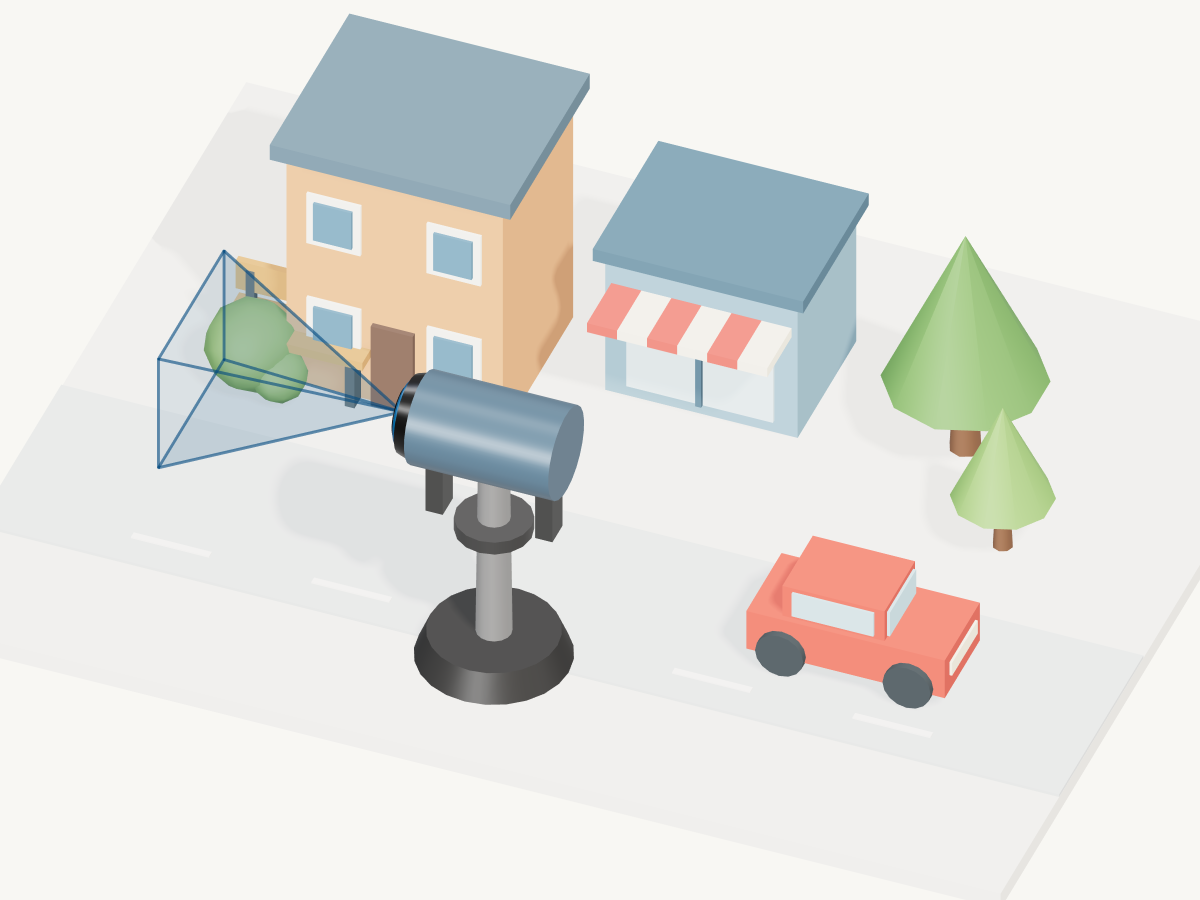
\includegraphics[width=6.6cm]{figures/img/main/three/renders/two_scales_ptz.png}};

% Pan wraps beneath the camera base, clear of the background buildings.
\draw[actionarr, <->] ($(ptz.center)+(-1.43,-1.52)$)
  .. controls ($(ptz.center)+(-1.43,-2.0)$) and ($(ptz.center)+(0.27,-2.0)$)
  .. node[actionlabel, below] {pan} ($(ptz.center)+(0.27,-1.52)$);
% Tilt follows the camera head's height, beside its rear pivot.
\draw[actionarr, <->] ($(ptz.center)+(0.1,0.58)$)
  .. controls ($(ptz.center)+(0.57,0.43)$) and ($(ptz.center)+(0.57,-0.27)$)
  .. node[actionlabel, right] {tilt} ($(ptz.center)+(0.1,-0.42)$);
% Zoom runs parallel to the lens direction, below the viewing cone.
\draw[actionarr, <->] ($(ptz.center)+(-1.3,-0.62)$) -- node[actionlabel, below, sloped] {zoom} ($(ptz.center)+(-2.45,-0.3325)$);

\node[titletext] (lefttitle) at ($(ptz.north)+(0,1.0)$) {Local scale exploration};
\node[captiontext] (leftsubtitle) at ($(lefttitle.center)+(0,-0.57)$) {where to look};
\node[captiontext, anchor=north] (leftcap) at ($(ptz.south)+(0,-0.25)$) {fixed position, redirects gaze};

% ---------- right: global scale (UAV) ----------
\node[imgnode, right=2.6cm of ptz] (uav) {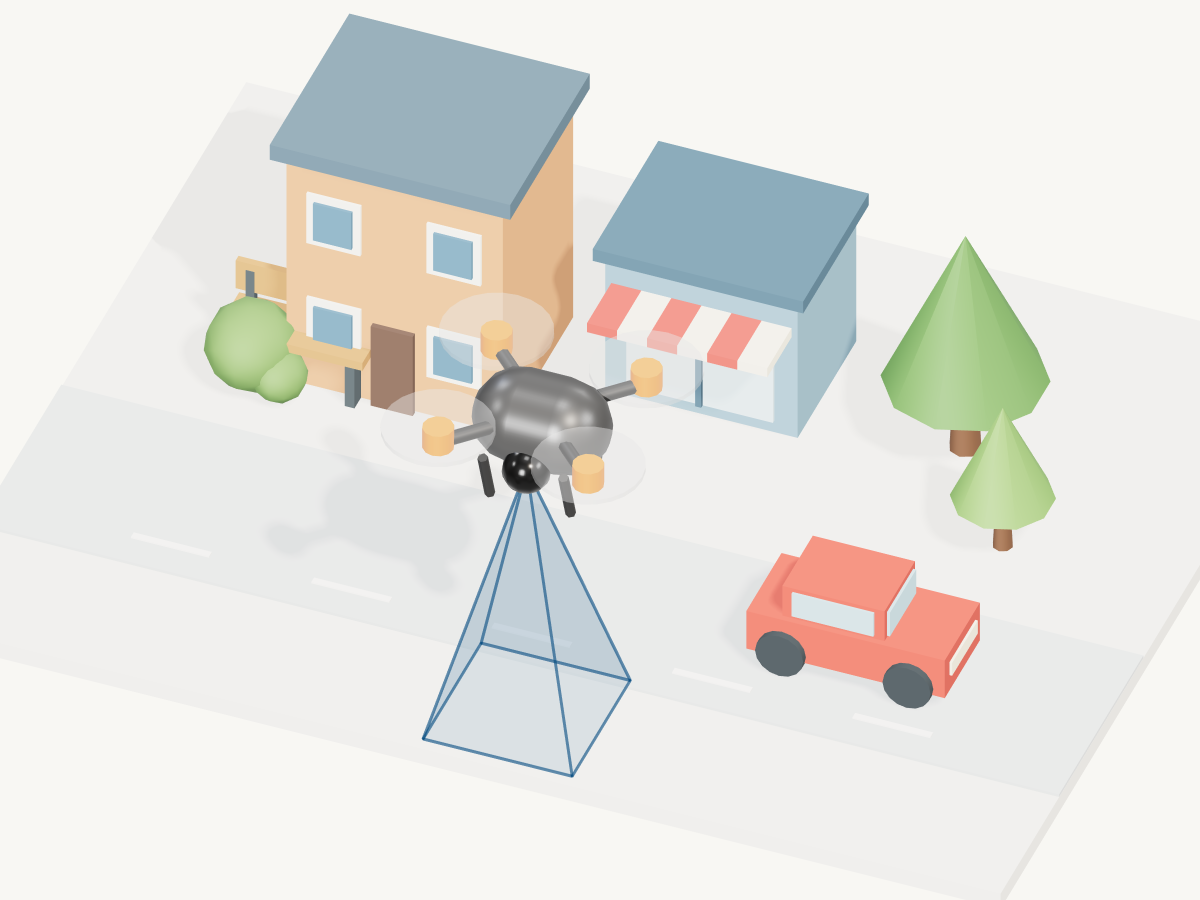
\includegraphics[width=6.6cm]{figures/img/main/three/renders/two_scales_uav.png}};

% Place the shared origin in clear foreground to the left of the UAV.
% Steep ground-plane diagonals keep all three directions distinct.
% Opposite directions are dashed; z has exactly the same x at both ends.
\coordinate (axesorigin) at ($(uav.center)+(-1.65,-1.25)$);
\draw[actionarr, dashed] (axesorigin) -- ($(axesorigin)+(-0.63,0.51)$);
\draw[actionarr, dashed] (axesorigin) -- ($(axesorigin)+(0.675,0.35)$);
\draw[actionarr, dashed] (axesorigin) -- ($(axesorigin)+(0,-0.95)$);
\draw[actionarr] (axesorigin) -- node[actionlabel, left, pos=0.75] {z} ($(axesorigin)+(0,1.3)$);
\draw[actionarr] (axesorigin) -- node[actionlabel, below left, pos=0.7] {x} ($(axesorigin)+(1.05,-0.85)$);
\draw[actionarr] (axesorigin) -- node[actionlabel, below, pos=0.7] {y} ($(axesorigin)+(-1.35,-0.70)$);
\fill[steelblue31119180!70!black] (axesorigin) circle[radius=1.2pt];

\node[titletext] (righttitle) at ($(uav.north)+(0,1.0)$) {Global scale exploration};
\node[captiontext] (rightsubtitle) at ($(righttitle.center)+(0,-0.57)$) {where to move};
\node[captiontext, anchor=north] (rightcap) at ($(uav.south)+(0,-0.25)$) {physically relocates through 3D space};

% Match the divider to the visible panel content; avoid caption padding.
\coordinate (divider) at ($(ptz.east)!0.5!(uav.west)$);
\draw[black!45, line width=0.4pt]
  (divider |- lefttitle.north) -- (divider |- leftcap.south);

\end{tikzpicture}%
\endgroup%
